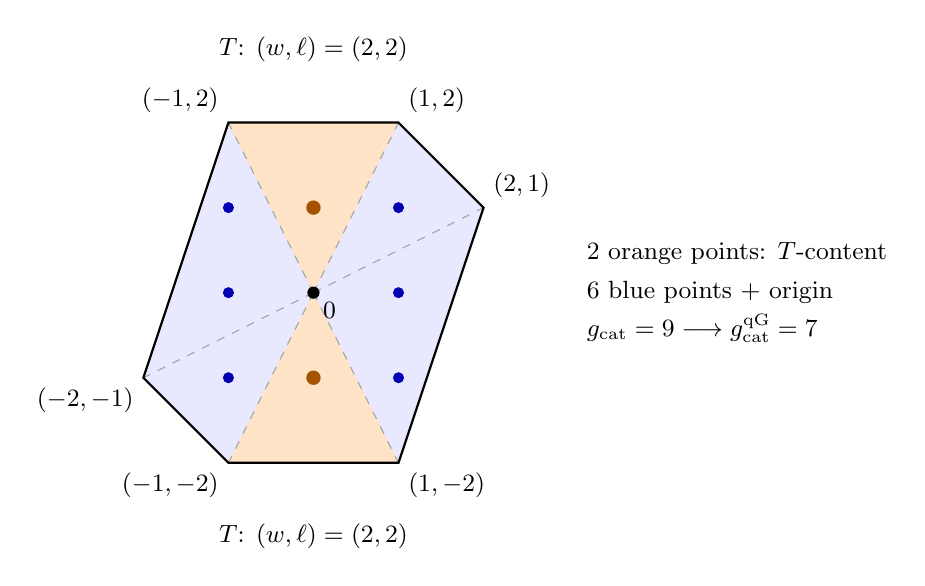
\begin{tikzpicture}[x=1.08cm,y=1.08cm,font=\small]
  \fill[blue!9] (2,1)--(1,2)--(-1,2)--(-2,-1)--(-1,-2)--(1,-2)--cycle;
  \fill[orange!22] (0,0)--(1,2)--(-1,2)--cycle;
  \fill[orange!22] (0,0)--(-1,-2)--(1,-2)--cycle;
  \foreach \horizontal/\vertical in {2/1,1/2,-1/2,-2/-1,-1/-2,1/-2}
    \draw[gray!70,dashed] (0,0)--(\horizontal,\vertical);
  \draw[thick] (2,1)--(1,2)--(-1,2)--(-2,-1)--(-1,-2)--(1,-2)--cycle;
  \foreach \horizontal in {-1,1}
    \foreach \vertical in {-1,0,1}
      \fill[blue!70!black] (\horizontal,\vertical) circle (2pt);
  \foreach \vertical in {-1,1}
    \fill[orange!65!black] (0,\vertical) circle (2.6pt);
  \fill (0,0) circle (2.2pt) node[below right] {$0$};
  \node[above] at (0,2.6) {$T$: $(w,\ell)=(2,2)$};
  \node[below] at (0,-2.6) {$T$: $(w,\ell)=(2,2)$};
  \node[above right] at (2,1) {$(2,1)$};
  \node[above right] at (1,2) {$(1,2)$};
  \node[above left] at (-1,2) {$(-1,2)$};
  \node[below left] at (-2,-1) {$(-2,-1)$};
  \node[below left] at (-1,-2) {$(-1,-2)$};
  \node[below right] at (1,-2) {$(1,-2)$};
  \node[anchor=west,align=left] at (3.1,0)
    {$2$ orange points: $T$-content\\[3pt]
     $6$ blue points $+$ origin\\[3pt]
     $g_{\mathrm{cat}}=9\longrightarrow g_{\mathrm{cat}}^{\mathrm{qG}}=7$};
\end{tikzpicture}